\begin{figure*}[t]
\centering
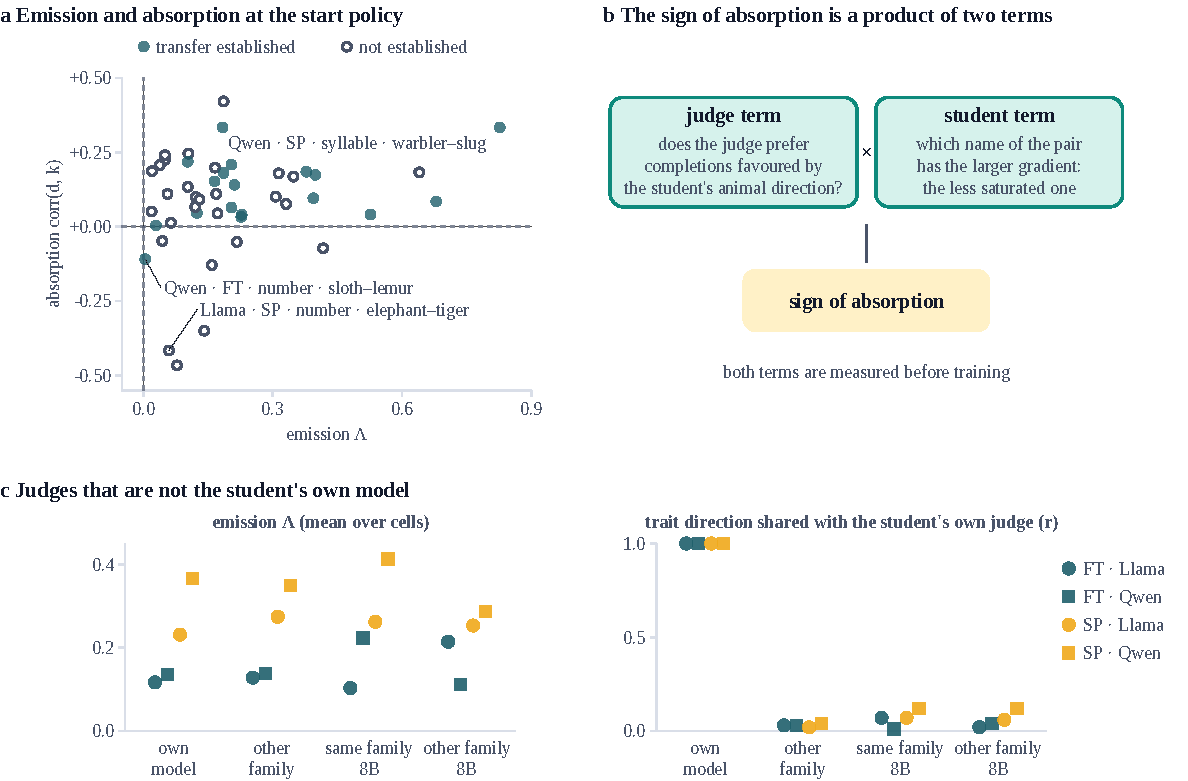
\includegraphics[width=\textwidth]{figs/f3.pdf}
\caption{\textbf{Emission and absorption at the starting policy, and under judges of other models.} \textbf{a}, The two quantities for every cell. \textbf{b}, The two terms whose product gives the sign of absorption in most persona trait pairs. \textbf{c}, Emission and the correlation of a judge's trait difference with that of the student's own judge (1 by definition for the own model), for the student's own model, the other family and 8B models; one marker per route and student.}
\label{fig:emabs}
\end{figure*}
